\chapter{Coding Approaches}

\section{Approaches to Cost Function}

When talking about TSP, the distance between nodes can be seen as the cost of the edges themselves.
These type of distances are defined by TSPLIB\cite{tsplib} and can be computed or precomputed and given as input inside the .tsp files, if they are not specified to begin with.
In this project only instances where the cost of the edges is represented by the distance between nodes will be considered, hence all the instances are made of a fully connected graph.
Since the edge costs are frequently accessed during the execution of the algorithms studied in this paper, the method to retrieve them must be as fast as possible.
It is possible to differentiate between two main categories of methods for retrieving edge costs.
\newline
The first one consist in computing the distance each time it is needed, while the second method involves computing all the distances at the beginning and storing each edge value inside the memory.
While the first is the simpleset and most straightforward implementation, it does come with a major drawback: speed.
Indeed there are more than a couple distance function defined by TSPLIB, almost every instance used during this project development included the need to compute the square root at some point.
The square root operation is an operation that is computationally intesive for computers that usually require iterative algorithms to compute.
Nowadays most modern computer architectures include an hardware dedicated square root instruction, which is many times faster compared to the interative algorithm, yet still takes a lot of time to execute.
\newline
The second category of methods eliminates this problem, since allowing to compute all cost at the start completely removes the need to use any kind of cost function down the line.
On paper this method is indeed the one which allows for the greatest speedup, but, unfortunatly that is not always the case.
Since the graphs under consideration are all fully connected, the number of edges increases in a quadratic relationship to the number of nodes.
Because of this the amount of memory needed to cache the cost of all edges is in the order of $O(n^2)$, as an example 137MB of memory is needed to store the edge costs of an instance with 6000 nodes.
Although it is still a small amount of memory compared to the amount of memory modern computers are equipped with, it is too much to fit a normal personal computer CPU cache.
It's well known that CPU cache is significantly faster than regular system memory, so being unable to fit the cost matrix inside the cache can negatively impact performance.
Cache misses occur when the data the CPU needs is not found in the fast-access cache memory and must be retrieved from the slower main memory.
This delay happens because the CPU has to pause its current operations to fetch the required data, leading to increased latency and reduced overall performance.
For this reason, it is very important to access the cost matrix in a manner that is as localized as possible; otherwise, the resulting algorithm speed can be severely affected.
\figurename{ \ref{fig:matrixBadIndex}} shows the performance difference caused by swapping the row and column indices when accessing a value of the matrix.

\begin{figure}[H]
    \centering
    \begin{tikzpicture}
        \begin{axis}[
            width=11cm, height=8cm,
            ymajorgrids=true,
            grid style={dashed,gray!30},
            xlabel=Instance size,
            ymin=0, ymax=6,
            ylabel=Relative iterations/s,
            legend style={at={(0.02,0.98)},anchor=north west,legend columns=-1},
            symbolic x coords={100,500,1000,5000,10000},
            log ticks with fixed point,
            xtick=data,
            % ytick={1,2,3,4,5},
            % yticklabels={100\%,200\%,300\%,400\%,500\%},
            ybar, 
                    ]
            \addplot[Blue,fill] table[x=n, y=cmpmatrix_badindex, col sep=semicolon] {csv/cmp_2opt.csv};
            \addplot[Red,fill] table[x=n, y=cmpmatrix_goodindex, col sep=semicolon] {csv/cmp_2opt.csv};
            \legend{Bad Indexing , Good Indexing}
        \end{axis}
    \end{tikzpicture}
    \caption{Comparison between good indexing and bad indexing performance} \label{fig:matrixBadIndex}
\end{figure}

Wanting to obtain greater speed we focused on optimizing one of the method explained above.
Since the second category methods are harder to optimize, more focus was given in finding a way to compute edge cost faster, thus optimizing the first category of methods.
The lingering issue lies in the time consumed by the square root operation, which can be streamlined through various optimizations like leveraging a lookup table.
To address this, the optimization utilized SIMD instructions known as AVX.
AVX (Advanced Vector Extensions) are a set of CPU instructions designed to perform parallel operations on multiple data elements simultaneously.
They enable faster processing by allowing a single instruction to operate on multiple data points, enhancing the efficiency of tasks such as mathematical computations and data manipulation.
Supporting operations between vectors of the size of 256 bits, AVX allows computing eight distance values, in floating-point 32-bit precision, simultaneously, enhancing computational efficiency.
Another advantage is that with this approach an easy and quick approximation of the square root becomes available.
By combining the instructions for reverse square root (rsqrt) and reciprocal (rpc), it is possible to achieve an approximation with a relative error smaller than $8 \times 10^{-4}$ in less than half the time required for a precise result.
This can be leveraged by performing the initial iterations of an algorithm like 2-Opt using the approximation, then switching to exact computation once the approximation can no longer identify optimizing moves.
However, coding an algorithm to utilize AVX is more complex, and not all algorithms can be optimized this way, as they may not be suitable for vectorized execution (e.g., Simulated Annealing).

\begin{figure}[H]
    \centering
    \begin{tikzpicture}
        \begin{axis}[
            width=11cm, height=8cm,
            ymajorgrids=true,
            grid style={dashed,gray!30},
            xlabel=Instance size,
            ymin=0, ymax=0.6,
            ylabel=,
            legend style={at={(0.02,0.98)},anchor=north west,legend columns=-1},
            symbolic x coords={100,500,1000,5000,10000},
            log ticks with fixed point,
            xtick=data,
            ytick={0,0.1,0.2,0.3,0.4,0.5,0.6},
            yticklabels={0\%,10\%,20\%,30\%,40\%,50\%,60\%},
            ybar, 
                    ]
            \addplot[Red,fill] table[x=n, y=cmpavx_approx, col sep=semicolon] {csv/cmp_2opt.csv};
            %\legend{}
        \end{axis}
    \end{tikzpicture}
    \caption{Speedup percentage given by using approximated search in 2opt} \label{fig:avxApprox}
\end{figure}

\subsection{Performance Comparison}

Comparing these three approaches is complex due to numerous factors, including the number of iterations the AVX approximated method performs before switching to the exact method, and the manner in which the cost matrix is accessed.
To minimize as much as possible these external factors, the data was gathered using multiple instances sizes as well as different cost functions.
\figurename{ \ref{fig:avxShowcase}} compares all approaches, scaling the to the basic one.
As expected, using the cost matrix method is faster than the basic method for small instances but loses its advantage as instance size increases.
Throughout the entire testing, the AVX approach consistently proved to be the fastest by a significant margin in every scenario.
However, it should be noted that the AVX method yielded unstable results on smaller instances, occasionally performing slower than the matrix method.

\begin{figure}[H]
    \centering
    \begin{tikzpicture}
        \begin{axis}[
            width=11cm, height=8cm,
            ymajorgrids=true,
            grid style={dashed,gray!30},
            xlabel=Instance size,
            ymin=0, ymax=9,
            ylabel=Relative iterations/s,
            legend style={at={(0.02,0.98)},anchor=north west,legend columns=-1},
            symbolic x coords={100,500,1000,5000,10000},
            log ticks with fixed point,
            xtick=data,
            % ytick={1,2,3,4,5,6,7,8},
            % yticklabels={100\%,200\%,300\%,400\%,500\%,600\%,700\%,800\%},
            ybar, 
                    ]
            \addplot[Blue,fill] table[x=n, y=cmp_base, col sep=semicolon] {csv/cmp_2opt.csv};
            \addplot[Red,fill] table[x=n, y=cmp_matrix, col sep=semicolon] {csv/cmp_2opt.csv};
            \addplot[Green,fill] table[x=n, y=cmp_avx, col sep=semicolon] {csv/cmp_2opt.csv};
            \legend{Basic,Matrix,AVX}
        \end{axis}
    \end{tikzpicture}
    \caption{Comparison of all three approaches in 2-Opt (measurment were taken using the best optimizations found for each approach)} \label{fig:avxShowcase}
\end{figure}


\section{Multithreading}

Multithreading is a programming technique that allows a computer program to perform multiple tasks concurrently, by dividing its execution into smaller threads of execution that can run independently.
In most of the algorithms implemented, multithreading consists in running the same code on different threads while using at random different data.
This is done by means of random seed, which means, giving to each thread running a different seed value so that it may find different solutions from the other running threads.
During this process the threads share between them the globally best solution found up to that point, so that, at the end of the execution, that solution will be given as output.
This type of implementation allows to have minimal interaction between threads, allowing a great benefit in term of iterations each second as shown in \figurename{ \ref{fig:multithreadNN}}.

Although this parallel design frequently appears in algorithm implementations, it is not always feasible to use this method.
For instance, algorithms that utilize CPLEX, which is inherently designed to run on multiple threads, present such a case.
Another example is the parallelization of the 2-Opt and the 3-Opt algorithms.
As the instance size increases, both methods require progressively more time to complete their computations.
Consequently, a straightforward parallel approach was developed.
The algorithm's scalability varies based on the instance size and the number of threads used, as shown in \figurename{ \ref{fig:multithread2opt}}.

\begin{figure}[H]
    \centering
    \begin{tikzpicture}
        \begin{axis}[
            % title={Multithreading speedup of 2-Opt parallel implementation},
            xlabel={Number of Threads},
            ylabel={Iterations/s Ratio},
            xmin=1, xmax=8,
            ymin=1, ymax=8,
            xtick={1,2,3,4,5,6,7,8},%,10,12,14,16,18,20},
            ytick={1,2,3,4,5,6,7,8},%,9,10,11,12,13,14,15,16},
            legend style={at={(0.98,0.02)},anchor=south east,legend columns=1},
            ymajorgrids=true,
            xmajorgrids=true,
            grid style=dashed,
        ]
        
        \addplot[Blue,mark=square] table[x=cores, y=nn100, col sep=semicolon] {csv/MT.csv};
        \addplot[Red,mark=o] table[x=cores, y=nn1000, col sep=semicolon] {csv/MT.csv};
        \addplot[Green,mark=triangle] table[x=cores, y=nn10000, col sep=semicolon] {csv/MT.csv};
        \addlegendentry{n=100}
        \addlegendentry{n=1000}
        \addlegendentry{n=10000}
            
        \end{axis}
    \end{tikzpicture}
	\caption{Multithreading speedup of Nearest Neighbor parallel implementation} \label{fig:multithreadNN}
\end{figure}


\begin{figure}[H]
    \centering
    \begin{tikzpicture}
        \begin{axis}[
            % title={Multithreading speedup of 2-Opt parallel implementation},
            xlabel={Number of Threads},
            ylabel={Iterations/s Ratio},
            xmin=1, xmax=8,
            ymin=0, ymax=8,
            xtick={1,2,3,4,5,6,7,8},
            ytick={0,1,2,3,4,5,6,7,8},
            legend style={at={(0.02,0.98)},anchor=north west,legend columns=2},
            ymajorgrids=true,
            xmajorgrids=true,
            grid style=dashed,
        ]
        
        \addplot[SkyBlue,mark=square] table[x=cores, y=2opt100, col sep=semicolon] {csv/MT.csv};
        \addplot[Red,mark=o] table[x=cores, y=2opt500, col sep=semicolon] {csv/MT.csv};
        \addplot[Purple,mark=triangle] table[x=cores, y=2opt1000, col sep=semicolon] {csv/MT.csv};
        \addplot[Blue,mark=diamond] table[x=cores, y=2opt5000, col sep=semicolon] {csv/MT.csv};
        \addplot[Green,mark=star] table[x=cores, y=2opt10000, col sep=semicolon] {csv/MT.csv};
        \addlegendentry{n=100}
        \addlegendentry{n=500}
        \addlegendentry{n=1000}
        \addlegendentry{n=5000}
        \addlegendentry{n=10000}
            
        \end{axis}
    \end{tikzpicture}
	\caption{Multithreading speedup of 2-Opt parallel implementation} \label{fig:multithread2opt}
\end{figure}

\section{Solution Representation}

Chosing the representation for the TSP solution the memory can be a challenge since there are many ways to do so.
We chose the \textbf{Path of Indices} as our primary representation.
This method involves using a single array whose size is equal to the number of nodes.
In this array, the indices of the nodes are stored, sorted by their occurrence in the tour.
This representation offers a main advantage that we relied on: the edges in the tour can be easily determined by examining the connections between nodes in adjacent positions in the solution.
This was useful during the development of the 2-Opt and 3-Opt algorithms, since this representation implicitly represents the edges of the tour, further data structures are not necessary.
Although it must be noted that in order to make use of this advantage the most, aspecially when using the AVX approach, the first node must be attached at the end of the array as well, to represent the last visited edge in the solution.
When not working with precomputed edges cost, it is also useful to keep the coordinates X and Y of the nodes sorted to match the solution order.
This last trick allowed for a great speedup in AVX computation, since a fast \textit{load} instruction could be used as opposed to a \textit{gather} function, which generates a sequence of instructions.
A small speedup was also observed on the Basic cost computation approach, probably due to the increase in the locality of memory access which caused a reduction in the overall number of cache misses.

\subsection{Cost Cache}

Throughout our implementations, many times an array of name \textbf{Cost Cache} appears.
As its name suggests, this simple array contains the cost of each of the edges in the solution, sorted according on the order in which edges are visited in the solution.

\begin{figure}[H]
    \centering
    \begin{tikzpicture}
        \begin{axis}[
            width=11cm, height=8cm,
            ymajorgrids=true,
            grid style={dashed,gray!30},
            xlabel=Instance size,
            ymin=0, ymax=0.5,
            ylabel=,
            legend style={at={(0.02,0.98)},anchor=north west,legend columns=-1},
            symbolic x coords={100,500,1000,5000,10000},
            log ticks with fixed point,
            xtick=data,
            ytick={0,0.1,0.2,0.3,0.4},
            yticklabels={0\%,10\%,20\%,30\%,40\%},
            ybar, 
                    ]
            \addplot[Blue,fill] table[x=n, y=cmpcc_avx_cc, col sep=semicolon] {csv/cmp_2opt.csv};
            \addplot[Red,fill] table[x=n, y=cmpcc_base_cc, col sep=semicolon] {csv/cmp_2opt.csv};
            \addplot[Green,fill] table[x=n, y=cmpcc_matrix_cc, col sep=semicolon] {csv/cmp_2opt.csv};
            \legend{Basic,Matrix,AVX}
        \end{axis}
    \end{tikzpicture}
    \caption{Speedup gained by each approach using the cost cache in 2-Opt} \label{fig:costCacheShowcase} 
\end{figure}

Born at first as a simple caching method to improve the speed of some algorithms, it now serves a vital role in the Tabu Search algorithm.

\begin{figure}[H]
    \centering
    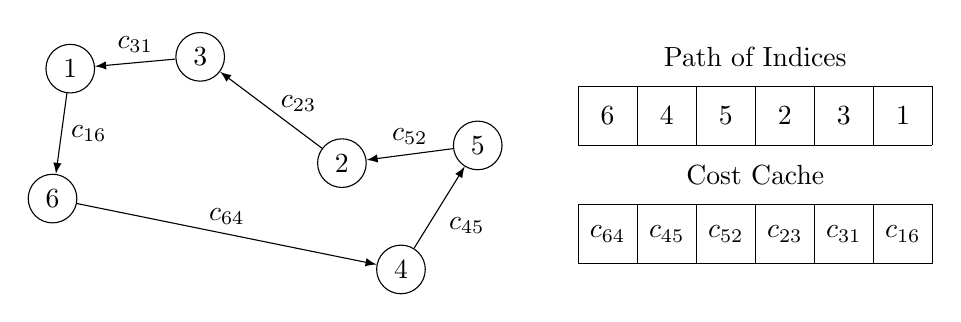
\begin{tikzpicture}[scale=0.75]
        \node[circle, draw, fill=white] (A) at (2.6, 4) {3};
        \node[circle, draw, fill=white] (B) at (0.4, 3.8) {1};
        \node[circle, draw, fill=white] (C) at (0.1, 1.6) {6};
        \node[circle, draw, fill=white] (D) at (6, 0.4) {4};
        \node[circle, draw, fill=white] (E) at (7.3, 2.5) {5};
        \node[circle, draw, fill=white] (F) at (5, 2.2) {2};
    
       \draw[-latex] (A) to node[above,] {$c_{31}$} (B);
		\draw[-latex] (B) to node[right] {$c_{16}$} (C);
		\draw[-latex] (C) to node[above] {$c_{64}$} (D);
		\draw[-latex] (D) to node[below right] {$c_{45}$} (E);
		\draw[-latex] (E) to node[above] {$c_{52}$} (F);
		\draw[-latex] (F) to node[above right, yshift=-4] {$c_{23}$} (A);
	
		\begin{scope}[shift={(9, 1.5)}]
			\draw (0,1) grid (6,2);
			\path (.5,.5) (0.5,1.5) node{$6$} ++(1,0) node{$4$} ++(1,0) node{$5$} ++(1,0) node{$2$} ++(1,0) node{$3$} ++(1,0) node{$1$};
			\draw (3,2.5) node{Path of Indices};
        \end{scope} 

		\begin{scope}[shift={(9, -0.5)}]
			\draw (0,1) grid (6,2);
			\path (.5,.5) (0.5,1.5) node{$c_{64}$} ++(1,0) node{$c_{45}$} ++(1,0) node{$c_{52}$} ++(1,0) node{$c_{23}$} ++(1,0) node{$c_{31}$} ++(1,0) node{$c_{16}$};
			\draw (3,2.5) node{Cost Cache};
        \end{scope}    

    \end{tikzpicture}
    \caption{Example of a Path of Indicies solution}
    \label{fig:solRepresentationExample}
\end{figure}

\subsection{Solution Cost Precision}

All the algorithms we implemented affect the total cost of the solution at some point, the ones that build the solution from scratch increase the cost of the tour as they iterate, while solution optimization oriented algorithm tend to decrease the overall cost by some amount at each iteration.
When used together with floating point precision, some problems might occur, especially when working on big instances;
We noticed this behavior when debugging the code of the 2-Opt algorithm:.
The earliest implementations of this algorithm in fact computed the overall cost offset of the optimization in floating point single precision (32 bits) and applied it to the overall cost which was represented as a double precision floating point (64 bits).
During the debugging phase a function to check the solution cost was called at each iteration.
That function simply followed the solution tour and increased the overall cost every time a new edge was visited.
Of course towards the end of the tour the overall cost would be much higher compared to the single edge cost that was going to be added, which means that, given a high enough instance size, the operation of computing the cost of the solution was bound to loose some precision in its representation.
This happens because of the very nature of the floating point representation.
Having said that it also stands to reason that by computing the cost the other way around would produce a ever so slightly different result.
This effect is even magnified when adding to the overall cost the cost offset value of some move, a value which is added to the sum of all the costs of the edges not, just a portion of them.
An easy fix for most of the isses caused by this precision problem is to recompute the cost of the solution each time.
The disadvantages of this fix are the fact that recomputing the cost each time is very computationally expensive, as well as the fact that the problem is not entirely solved, since the same solution cost computed backwards is not guaranteed to be the same.
We took a different approach to remove the issue entirely: we made the cost of the solution to be represented by a fixed point variable of 128 bits.
While keeping the edge costs in floating point variables, when converting to the fixed point value truncation gets rid of any possible discrepancies.
The size of 128 bits was to address a very large range of instances, since some may have nodes very close to each other which translates into small edge costs overall while other may be the opposite.
We set the separation between integer and fractional part to be in the middle, giving 64 bits for each the integer and fractional parts.